\documentclass[11pt,letter]{ivoa}
\input tthdefs

\usepackage{todonotes}
\usepackage{listings}
\lstloadlanguages{XML}
\lstset{flexiblecolumns=true,basicstyle=\small,tagstyle=\ttfamily}


\title{Data Access Layer Interface}

\ivoagroup{Data Access Layer Working Group}

\author{Patrick Dowler}
\author{Markus Demleitner}
\author{Mark Taylor}
\author{Doug Tody}

\editor{Patrick Dowler}

\previousversion[http://www.ivoa.net/Documents/DALI/1.1]{DALI-1.1}
\previousversion[http://www.ivoa.net/Documents/DALI/1.0]{DALI-1.0}

\begin{document}

\begin{abstract}
This document describes the Data Access Layer Interface (DALI). DALI defines
the base web service interface common to all Data Access Layer (DAL) services.
This standard defines the behaviour of common resources, the meaning and use of
common parameters, success and error responses, and DAL service registration.
The goal of this specification is to define the common elements that are shared
across DAL services in order to foster consistency across concrete DAL service
specifications and to enable standard re-usable client and service
implementations and libraries to be written and widely adopted.
\end{abstract}

\section{Introduction}
The Data Access Layer Interface (DALI) defines resources, parameters, and
responses common to all DAL services so that concrete DAL service specifications
need not repeat these common elements.

\subsection{Role within the VO Architecture}
DALI defines how DAL service specifications use other IVOA standards as well as
standard internet designs and protocols. Fig.~\ref{fig:archdiag} shows the role
this document plays within the IVOA architecture \citep{2021ivoa.spec.1101D}.

\begin{figure}
\centering

% Get the architecture diagram from the TCG chair
% http://wiki.ivoa.net/twiki/bin/view/IVOA/IvoaTCG
% If they give you a PDF, for now dumb it down to a png by
% convert -antialias -density 72x72 archdiag.pdf archdiag.png
% Oh -- Notes don't need this; you'd have to remove archdiag.png
% from FIGURES in the Makefile, too.

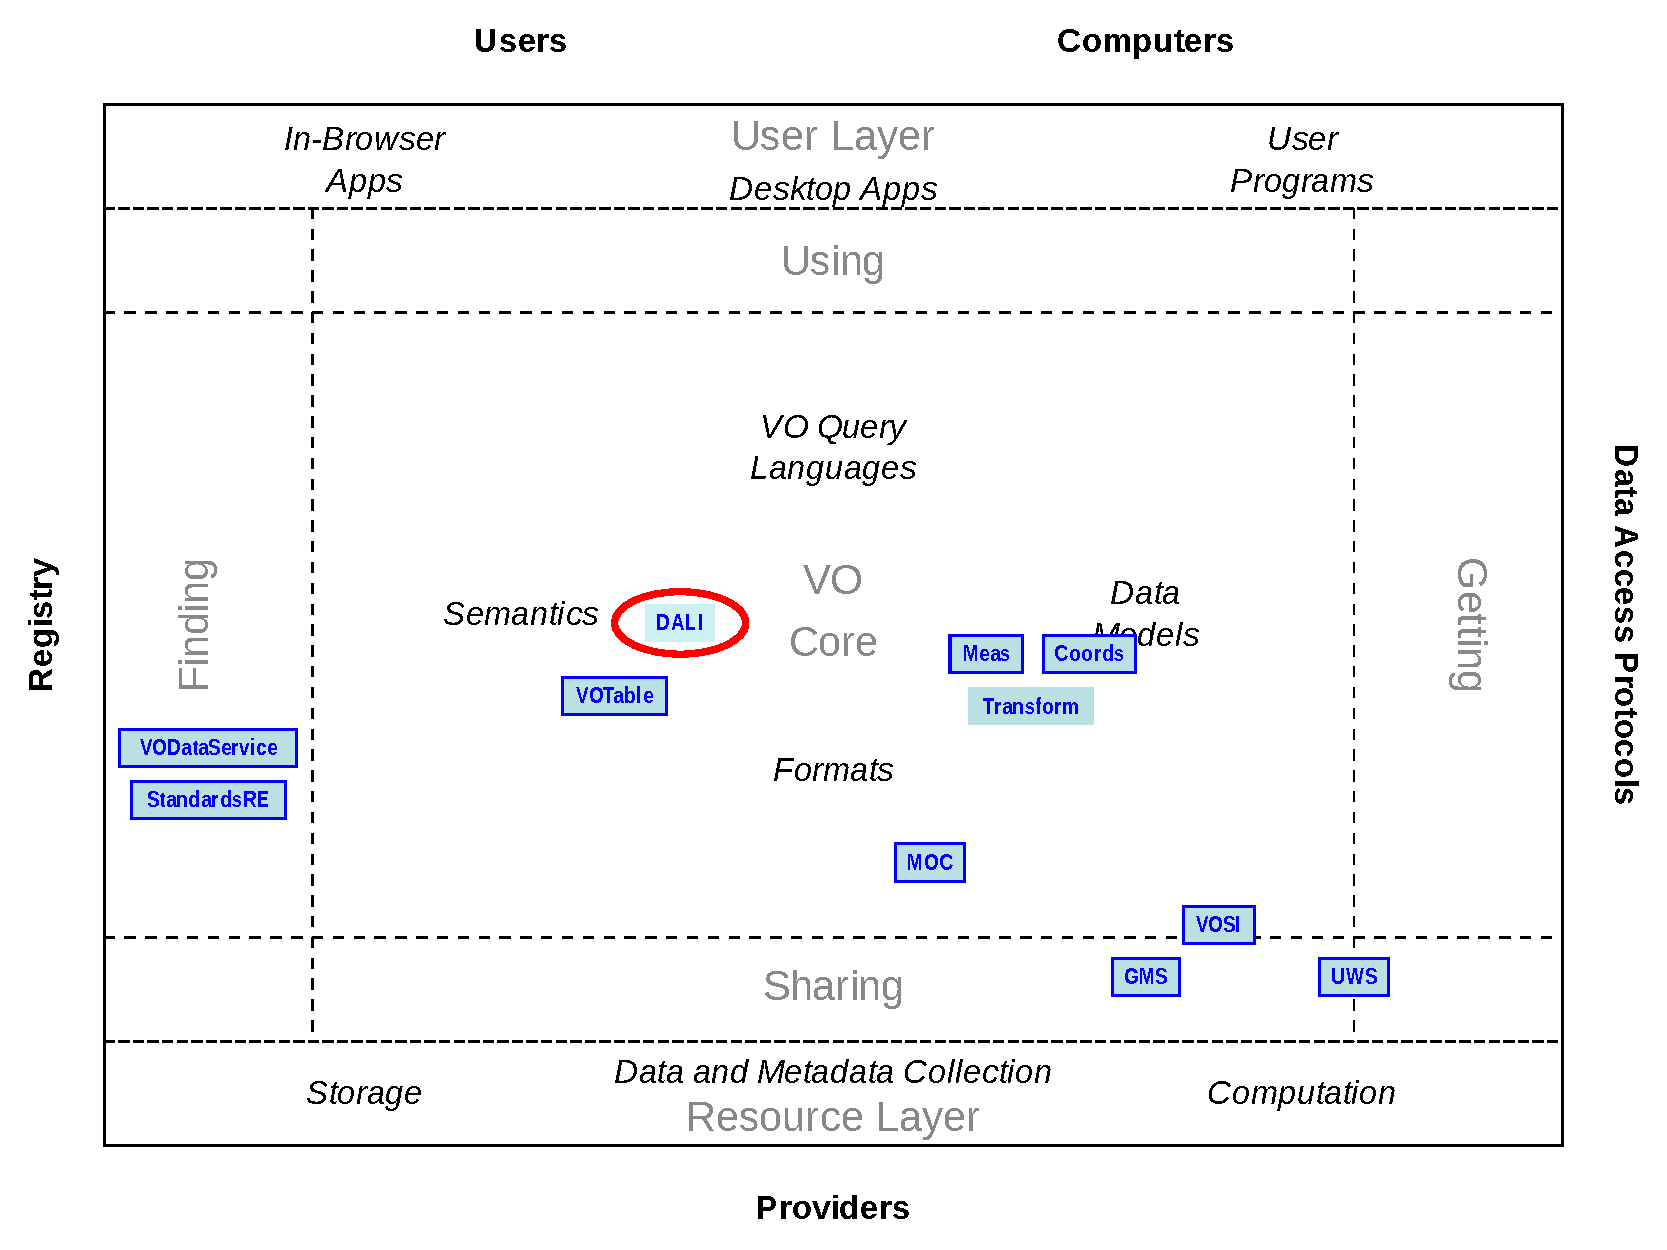
\includegraphics[width=0.9\textwidth]{role_diagram.pdf}
\caption{Architecture diagram for this document}
\label{fig:archdiag}
\end{figure}

Astronomical coordinate values accepted and returned by DAL services use a
string representation of the Space-Time Coordinates \citep{2007ivoa.spec.1030R} data
model. The
concrete DAL service specification defines whether the returned resources are
serializations of a particular standard data model. For preserving backwards
compatibility or to enable service-specific use cases, the concrete DAL service
specification may explicitly specify the use of ad-hoc Utypes.

A registry extension schema, usually extending VODataService \citep{2021ivoa.spec.1102D},
may be used to
describe the capabilities of a DAL service. This schema is used within the
VOSI-capabilities \citep{2017ivoa.spec.0524G} resource and in registry records for the
service.

\subsection{Example Usage of the DALI Specification}
The DALI specification defines common elements that make up Data Access Layer
(DAL) services. DAL service specifications will refer to the sections in this
document by name rather than include all the explanatory text. For example,
suppose a document defines a service that stacks FITS images asynchronously, the
specification could say that the service has the following resources:


\begin{itemize}
\item a DALI-async resource that accepts one or more UPLOAD parameters
(section~\ref{sec:UPLOAD}) where the resources are FITS images; the resource
could also define a fixed set of error messages for anticipated failure modes

\item a VOSI-availability resource (section~\ref{sec:vosi-availability})

\item a VOSI-capabilities resource (section~\ref{sec:vosi-capabilities}) conforming
to a specified registry extension schema
\end{itemize}

\noindent
and would have to define the registry extension schema to be used to register
services and to implement the VOSI-capabilities resource. Most of the service
specification would be in defining the semantics (possibly controllable via
additional input parameters) of the computations to be performed and in defining
the extension schema to describe service functionality and limits (e.g., maximum
input or result image sizes, result retention time and policies). The registry
extension schema may be part of the service specification or a separate
document.

\section{Resources}
\label{sec:resources}
DAL services are normally implemented as HTTP REST \citep{fielding00}
web services, although
other transport protocols could be used in the future. The primary resource in
a DAL service is a job. A DAL job is defined by parameters
(section~\ref{sec:parameters}) and
can be executed either synchronously or asynchronously. A concrete service
specification defines the job parameters and the manner of execution is defined
by separate resources below.

In addition to job list resources, DAL services also implement several Virtual
Observatory Support Interface \citep{2017ivoa.spec.0524G} resources to describe
service availability, capabilities, and content.

A concrete DAL service must define at least one DALI-async or DALI-sync
resource. It may define both with the same job semantics (e.g. TAP-1.0
\citep{2010ivoa.spec.0327D}) or it may define one with one kind of job and the other with a
separate kind of job (a service that does some things synchronously and others
asynchronously).

The following table summarises the resources that are required in all concrete
DAL service specifications (and thus in all DAL services) and which kinds of
resources are defined and specified as required or optional in a concrete
specification.


\begin{tabular}{l l l l l}
\sptablerule
\textbf{resource type} & \textbf{resource name} & \textbf{required} \\
\sptablerule
DALI-sync & service specific & service specific & \\
DALI-async & service specific & service specific & \\
DALI-examples & /examples & no & \\
VOSI-availability & service specific & no & \\
VOSI-capabilities & /capabilities & registered & \\
VOSI-tables & service specific & service specific & \\
\sptablerule
\label{tab:resources}
\end{tabular}

The resource name is the path (relative to the base URL of the service). All implemented
DALI and VOSI endpoints must be siblings, except for VOSI-availability (see below);
concrete service specifications may constrain the names of these endpoints further.
The relative path limitation enables a client with just the URL for a single endpoint to
find the VOSI-capabilities endpoint and then discover all the capabilities
provided by the service.

A VOSI-capabilities endpoint is required for services registered in the IVOA registry system;
the VOSI-capabilities endpoint is optional for services that are not registered
or only included as auxiliary capabilities (e.g. of a data collection resource).

The URL for the VOSI-availability is not constrained; it may be a sibling (e.g. /availability)
or it may be hosted on a different server (e.g. VOSI-availability may be implemented as a
completely external resource that tests the service from the user perspective).

A simple query-only DAL service like ConeSearch can be easily described as
having a single DALI-sync resource where the job is a query and the response is
the result of the query.

\subsection{Asynchronous Execution: DALI-async}
\label{sec:dali-async}
Asynchronous resources are resources that represent a list of asynchronous jobs
as defined by the Universal Worker Service (UWS) pattern \citep{2016ivoa.spec.1024H}.
Requests can
create, modify, and delete jobs in the job list. UWS also specifies special
requests to modify the phase of the job (cause the job to execute or abort).

As specified in UWS, a job is created by using the HTTP POST method to modify
the job list. The response will always be an HTTP redirect (status code 303) and
the Location (HTTP header) will contain the URL to the job.

\begin{verbatim}
POST http://example.com/base/async-jobs
\end{verbatim}

The response will include the HTTP status code 303 (See Other) and a header
named Location with a URL to the created job as a value, for example:

\begin{verbatim}
Location: http://example.com/base/async-jobs/123
\end{verbatim}

The job description (an XML document defined by the UWS schema) can always be
retrieved by accessing the job URL with the HTTP GET method:

\begin{verbatim}
GET http://example.com/base/async-jobs/123
\end{verbatim}

\begin{lstlisting}[language=XML,basicstyle=\footnotesize]
<?xml version="1.0" encoding="UTF-8"?>
<uws:job xmlns:uws="http://www.ivoa.net/xml/UWS/v1.0">
  <uws:jobId>123</uws:jobId>
  <uws:runId>test</uws:runId>
  <uws:ownerId xsi:nil="true" />
  <uws:phase>PENDING</uws:phase>
  <uws:quote>2013-01-01T12:34:56</uws:quote>
  <uws:startTime/>
  <uws:endTime/>
  <uws:executionDuration>600</uws:executionDuration>
  <uws:destruction>2013-02-01T00:00:00</uws:destruction>
  <uws:parameters>
    <uws:parameter id="LANG">ADQL</uws:parameter>
    <uws:parameter id="REQUEST">doQuery</uws:parameter>
    <uws:parameter id="QUERY">select * from tab</uws:parameter>
  </uws:parameters>
  <uws:results/>
</uws:job>
\end{lstlisting}

In addition to the UWS job metadata, DAL jobs are defined by a set of
parameter-value pairs. The client may include parameters in the initial POST
that creates a job or it may add additional parameters by a POST to the current
list of parameters, for example:

\begin{verbatim}
http://example.com/base/async-jobs/123/parameters
\end{verbatim}

DALI-async resources may provide other ways to interact with jobs as specified
in current or future UWS specifications, with the following exception: the
UWS-1.0 standard may be interpreted to allow POSTing of job parameters to the
job URL, but DALI-async resources must not accept job parameters at this URL.

Job parameters may only be POSTed while the job is in the PENDING phase; once
execution has been requested and the job is in any other phase, job parameters
may not be modified.

A concrete DAL service specification will specify zero or more asynchronous job
submission resources and whether they are mandatory or optional. It may mandate
a specific resource name to support simple client use, or it can allow the
resource name to be described in the service metadata (Section~\ref{sec:vosi-capabilities}).

\subsection{Synchronous Execution: DALI-sync}
\label{sec:dali-sync}
Synchronous resources are resources that accept a request (a DAL job
description) and return the response (the result) directly. Synchronous requests
can be made using either the HTTP GET or POST method. If a specific type of job
is exposed through both DALI-async and DALI-sync resources (e.g. TAP queries),
then the parameters used to specify the job are the same for  this pair of
(synchronous and asynchronous) jobs. Service specifications may also specify
different types of jobs on different resources, which would have different job
parameters.

A synchronous job is created by a GET or POST request to a synchronous job list,
executed automatically, and the result returned in the response. The web service
is permitted to split the operation of a synchronous request into multiple HTTP
requests as long as it is transparent to standard clients. This means that the
service may use HTTP redirects (status code 302 or 303) and the Location header
to execute a synchronous job in multiple steps. For example, a service may

\begin{itemize}
\item immediately execute and return the result in the response, or
\item the response is an HTTP redirect (status code 303) and the Location (HTTP
header) will contain a URL; the client accesses this URL with the HTTP GET
method to execute the job and get the result
\end{itemize}

Clients must be prepared to get redirects and follow them (using normal HTTP
semantics) in order to complete requests.

A concrete DAL service specification will specify zero or more synchronous job
submission resources and whether they are mandatory or optional. It may mandate
a specific resource name to support simple client use, or it can allow the
resource name to be described in the service capability metadata 
(Section~\ref{sec:vosi-capabilities}).

\subsection{DALI-examples}
\label{sec:dali-examples}
The DALI-examples resource returns a document with usage examples or similar
material to the user. In DAL services, this resource is always accessed as a
resource named examples that is a child of the base URL for the service. The
following specification is intended to make sure the content is usable for both
machines and humans. As such, the DALI-examples resource contains additional
markup conforming to the RDFa 1.1 Lite \citep{std:RDFaLite11} specification,
which defines the
following attributes: \xmlel{vocab}, \xmlel{typeof}, \xmlel{property},
\xmlel{resource}, and \xmlel{prefix} (although we
do not include any use of the \xmlel{prefix} attribute).

The DALI-examples capability identifier is:
$$
\hbox{\nolinkurl{ivo://ivoa.net/std/DALI#examples}}
$$

DAL services may implement the /examples resource and include it in the
capabilities described by the VOSI-capabilities resource 
(Section~\ref{sec:vosi-capabilities}); if they
do not, retrieving its URL must yield a 404 HTTP error code.

The document at /examples must be well-formed XML. This restriction is imposed
in order to let clients parse the document using XML parsers rather than
much more complex parsers (e.g. HTML5 parsers). It is therefore advisable to
author it in XHTML, although this specification does not prescribe any document
types.

The document should be viewable with ``common web browsers''. Javascript or CSS
must not be necessary to find and interpret the elements specified below.  Apart
from that, service operators are free to include whatever material or styling
they desire in addition and within the example elements defined here.

The elements containing examples must be descendants of an element that has a
\xmlel{vocab} attribute with the value as shown below:

\begin{lstlisting}[language=XML]
<div vocab="http://www.ivoa.net/rdf/examples#">
...
</div>
\end{lstlisting}

The URI in the \xmlel{vocab} attribute resolves to an IVOA vocabulary of
concepts useful for describing examples.  That vocabulary complies to
Vocabularies in the VO version 2 \citep{2021ivoa.spec.0525D}.   The
values of the \xmlel{property} attributes below are described in it, and
the concept URIs formed according to RDFa rules resolve to elements
within it, which may be useful for documentation purposes.  Clients
purely interested in presenting the examples to their users usually have
no reason to retrieve the vocabulary.

No other \xmlel{vocab} attributes are allowed in the document. Each example resides in
an element that has a \xmlel{typeof} attribute with the value
\emph{example}. All such elements
must have an \xmlel{id} attribute to allow external referencing via fragments and a
\xmlel{resource} attribute with a reference pointing to the element itself. As an
example,

\begin{lstlisting}[language=XML]
<div id="x" resource="#x" typeof="example"> ... </div>
\end{lstlisting}

\noindent located inside the element having the \xmlel{vocab} attribute would
contain an example referable via the \emph{x} fragment identifier. The
\xmlel{div} element is
a suitable HTML element to hold an example.

The content of the example is expressed using the \xmlel{property} attribute. For
DALI-examples, we define the following values for the \xmlel{property} attribute:

\begin{itemize}
\item \emph{name}
\item \emph{capability}
\item \emph{generic-parameter}
\item \emph{continuation}.
\end{itemize}

Each example must include one
name.  DAL service specifications may define additional
properties so they can mark up additional information in their examples
using the procedures described in Vocabularies in the VO 2.  For
instance, TAP has introduced the notions of \emph{query} and \emph{table}.

In principle, any element permitted by the document type can include the RDFa
attributes, so authors may re-use existing markup intended for display.
Alternatively, the \xmlel{span} element is a good choice when the example values are
included in surrounding text and the author does not want any special rendering
to be applied by the machine-readable additions.

To maintain compatibility with mainstream RDFa tools, extra care is
necessary with elements that have \xmlel{src} or \xmlel{href}
attributes.  According to RDFa rules, in such cases the object of the
relationship is the linked entity rather than the element content.
While this is intended in some cases -- see the continuation property
below -- this will lead to erroneous interpretations in the typical
case.

For instance,

\begin{lstlisting}[language=XML]
<!-- Wrong! -->
<div id="x" resource="#x" typeof="example">
<p>The case of <a property="name"
  href="http://object-resolver.edu/M42">Messier 42</a> is special.</p>
</div>
\end{lstlisting}

\noindent
would imply that the name of the example \texttt{x} is
\nolinkurl{http://object-resolver.edu/M42} rather than just ``Messier
42''.  Full RDFa offers the \xmlel{content} attribute to allow correct
markup even in the presence of \xmlel{href} attributes, but since DALI
examples are restricted to RDFa lite, this cannot be used.

The rule of thumb is to only use elements with links when the
relationship's object actually is a linked document or entity (for the
terms given here, this is only true for continuation).  If document
authors wants to express a link with the relationship's object anyway,
they will have to restructure their texts (which typically will also
yield better link semantics).  For instance, the example above could be
written as:

\begin{lstlisting}[language=XML]
<div id="x" resource="#x" typeof="example">
<p>The case of <span property="name">Messier 42</span> (<a
  href="http://object-resolver.edu/M42">M42 at object resolver</a>)
  is special.</p>
</div>
\end{lstlisting}

\subsubsection{name property}

The content of this element must be plain text (i.e., no child
elements) and
should be suitable for display within a
space-limited label in user interface and still give some idea about the meaning
of the example.  In XHTML, a head element (\xmlel{h2}, say) would usually be a good
choice for the example name, for example:

\begin{lstlisting}[language=XML]
<h2 property="name">Synchronous TAP query</h2>
\end{lstlisting}

\subsubsection{capability property}

The capability property for an example specifies which service capability the
example is to be used with by giving, in plain text, the standards URI
as given in the respective capability's \xmlel{standardID} attribute.
For example, if the text is describing how to use a
SODA-1.0 service, the example could contain:

\begin{lstlisting}[language=XML]
<span property="capability">ivo://ivoa.net/std/SODA#sync-1.0</span>
\end{lstlisting}

IVOA standard service capabilities are defined as URIs,  so example documents
may want to show the URI or show more user-friendly text depending on the
expected audience for the document. For specifications that do not define
specific capability identifiers, the IVOID for the specification itself should
be used.

\subsubsection{generic-parameter property}

Request parameters are included within the example by using the
generic-parameter property. The element must also be assigned a
\xmlel{typeof} attribute
with value of \emph{keyval}. Within this element, the document must include a pair of
elements with \xmlel{property} attributes valued key and value, where the plain-text content are
the parameter name and value respectively. Multiple generic-parameter(s) are
permitted, for example:

\begin{lstlisting}[language=XML]
<span property="generic-parameter" typeof="keyval">
   <span property="key">REQUEST</span>
   <span property="value">doQuery</span>
</span>
<span property="generic-parameter" typeof="keyval">
   <span property="key">LANG</span>
   <span property="value">ADQL</span>
</span>
<span property="generic-parameter" typeof="keyval">
   <span property="key">QUERY</span>
   <span property="value">SELECT * from tap_schema.tables</span>
</span>
\end{lstlisting}

\subsubsection{continuation property}

If the examples are spread over multiple linked documents, the links to
documents with additional examples must be within the parent element defining
the \xmlel{vocab} attribute and the link elements must contain the following additional
attributes:  a \xmlel{property} attribute with the value
\emph{continuation}, a \xmlel{resource}
attribute with an empty value (referring to the current document), and
the \xmlel{href}
attribute with the URL of another document formatted as above (i.e. another
collection of examples that clients should read to collect the full set of
examples).

\begin{lstlisting}[language=XML,basicstyle=\footnotesize]
<div vocab="http://www.ivoa.net/rdf/examples#">
  <div id="x" resource="#x" typeof="example">
    ...
  </div>
  <a property="continuation"
     href="simple_examples.html">Simple examples</a>
  <a property="continuation"
     href="fancy_examples.html">Fancy examples</a>
</div>
\end{lstlisting}

In the above example, the two linked documents would also contain some element
with a vocab and examples as described above.

\subsection{Availability: VOSI-availability}
\label{sec:vosi-availability}
VOSI-availability \citep{2017ivoa.spec.0524G} defines a simple web resource that
reports on the current ability of the service to perform.

If the VOSI-availability resource is implemented a description
of this capability must be provided in the VOSI-capabilities document.
The VOSI-availability resource is
intended to respond with a dynamically generated document describing the current state of the service
operation, e.g.:

\begin{lstlisting}[language=XML,basicstyle=\footnotesize]
<?xml version="1.0" encoding="UTF-8"?>
<vosi:availability
  xmlns:vosi="http://www.ivoa.net/xml/VOSIAvailability/v1.0">
  <vosi:available>true</vosi:available>
  <vosi:note>service is accepting queries</vosi:note>
</vosi:availability>
\end{lstlisting}

\subsection{Capabilities: VOSI-capabilities}
\label{sec:vosi-capabilities}
VOSI-capabilities \citep{2017ivoa.spec.0524G} defines a simple web resource that
returns an XML document
describing the service. In  DAL services, this resource is always accessed as a
resource named capabilities that is a child of the base URL for the service. The
VOSI-capabilities should describe all the resources exposed by the service,
including which standards each resource implements.

All registered DAL services must implement the /capabilities resource. The following
capabilities document shows the capabilities and tables VOSI resources
and a TAP base resource:

\begin{lstlisting}[language=XML,basicstyle=\footnotesize]
<?xml version="1.0" encoding="UTF-8"?>
<vosi:capabilities
   xmlns:vosi="http://www.ivoa.net/xml/VOSICapabilities/v1.0"
   xmlns:xsi="http://www.w3.org/2001/XMLSchema-instance"
   xmlns:vod="http://www.ivoa.net/xml/VODataService/v1.1">

  <capability standardID="ivo://ivoa.net/std/VOSI#capabilities">
    <interface xsi:type="vod:ParamHTTP" version="1.0">
      <accessURL use="full">
         http://example.com/tap/capabilities
      </accessURL>
    </interface>
  </capability>

  <capability standardID="ivo://ivoa.net/std/VOSI#tables">
    <interface xsi:type="vod:ParamHTTP" version="1.0">
      <accessURL use="full">
        http://example.com/tap/tables
      </accessURL>
    </interface>
  </capability>

  <capability xmlns:tr="http://www.ivoa.net/xml/TAPRegExt/v1.0"
    standardID="ivo://ivoa.net/std/TAP" xsi:type="tr:TableAccess">
    <interface xsi:type="vod:ParamHTTP" role="std" version="1.0">
      <accessURL use="full">
           http://example.com/tap/
      </accessURL>
    </interface>
    <!-- service details from TAPRegExt go here -->
  </capability>
</vosi:capabilities>
\end{lstlisting}

Note that while this example shows the use of a registry extension schema (the
inline \verb|xmlns:tr="http://www.ivoa.net/xml/TAPRegExt/v1.0"| in the last capability
element) this is not required; services may be registered and described without
such an extension. The use of \xmlel{standardID} -- which should contain the
IVOID of
the standard a capability adheres to -- does not imply a particular (or any)
\xmlel{xsi:type} be included.

\subsection{Tables: VOSI-tables}
\label{sec:vosi-tables}
VOSI-tables \citep{2017ivoa.spec.0524G} defines a simple web resource that returns an
XML document
describing the content of the service. The document format is defined by the
VOSI \citep{2017ivoa.spec.0524G} standard and allows the service to
describe their content
as a tableset: schemas, tables, and columns.

A concrete DAL service specification will specify if the VOSI-tables resource is
permitted or required and may restrict the resource name or location.
Since DAL services with a VOSI-tables resource will specify
in the capabilities which version they are using, DAL services can make use of
new versions without change to the DAL service specification.

\section{Data Types and Literal Values}
\label{sec:xtypes}
In this section we specify how values are to be expressed. These literal values
are used as input or output from DAL services: as parameter values when
invoking services, as data values in response documents (e.g. VOTable),
etc. We define some general purpose values for the \xmlel{xtype} attribute of
the VOTable \xmlel{FIELD} and \xmlel{PARAM} elements for simple
structured values: \emph{timestamp}, \emph{interval},
\emph{hms}, \emph{dms},
\emph{point}, \emph{circle}, \emph{range}, \emph{polygon}, \emph{moc},
\emph{shape}, \emph{multishape}, \emph{uri}, and \emph{uuid} (see below).

In the following, where we say \verb|datatype="char"| we also allow the VOTable 
\verb|datatype="unicodeChar"|. Where we say \verb|arraysize="*"| we also allow 
providers to be more explicit by using a fixed size (e.g. \verb|20|) or fixed 
with a limit (e.g. \verb|20*|) when applicable.

In the following, where we say "VOTable type metadata", we mean either VOTable 
\xmlel{FIELD} or \xmlel{PARAM} elements.

Services may use non-standard \xmlel{xtype} values for non-standard datatypes, but if they
do so they should include a simple prefix (a string followed by a colon
followed by the non-standard xtype) so client software can easily determine
if a value is standard or not. For example, an \xmlel{xtype} for a
non-standard 3D-vector might be \emph{geom:vector3d}.

\subsection{Numbers}
Integer and real numbers must be represented in a manner consistent with the
specification for numbers in VOTable \citep{2019ivoa.spec.1021O}.  When used as
values in service parameters, the serialization for \xmlel{TABLEDATA} must be used.

\subsection{Boolean}
Boolean values must be represented in a manner consistent with the
specification for boolean in VOTable \citep{2019ivoa.spec.1021O}. When used as
values in service parameters, the serialization for \xmlel{TABLEDATA} must be used.

\subsection{Timestamp}
Timestamp values serialised in VOTable or described in service parameters must have 
the following VOTable type metadata:

\begin{verbatim}
datatype="char" arraysize="*" xtype="timestamp"
\end{verbatim}

\noindent
Date and time values must be represented  using the convention established for
FITS \citep{std:FITS} and STC \citep{2007ivoa.spec.1030R} for astronomical times:

\begin{verbatim}
YYYY-MM-DD['T'hh:mm:ss[.SSS]]
\end{verbatim}

\noindent
where the T is a character separating the date and time components. The time
component is optional, in which case the T separator is not used. Fractions of a
second are permitted but not required. For example:

\begin{verbatim}
2000-01-02T15:20:30.456
2001-02-03T04:05:06
2002-03-04
\end{verbatim}

\noindent
are all legal date or date plus time values. Astronomical values never
include a time zone indicator. However, values that
are civil in nature (e.g. when some processing was completed, when some record
was last modified) may include the time zone indicator Z to explicitly specify
the UTC time zone. Civil times conform to:

\begin{verbatim}
YYYY-MM-DD['T'hh:mm:ss[.SSS]['Z']]
\end{verbatim}

\noindent
where the optional Z character indicates the value is UTC. For example:

\begin{verbatim}
2000-01-02T15:20:30.456Z
2000-01-02T15:20:30Z
\end{verbatim}

\noindent
are valid civil time values. In cases where time values may be
expressed using Julian Date (JD) or Modified Julian Date (MJD), these follow the
rules for double precision numbers above and may have additional metadata as
described in the VOTable standard \citep{2019ivoa.spec.1021O}. All date-time values (formatted string, JD,
and MJD) shall be interpreted as referring to time scale UTC and time reference
position UNKNOWN, unless either or both of these are explicitly specified to be
different \citep{2007ivoa.spec.1030R}.

Note that the format used here is very close to the standard ISO8601 timestamp
format except with respect to timezone handling. ISO8601 requires a Z character
at the end of the string when the timezone is UTC; here, we follow the FITS
\citep{std:FITS} convention for astronomical values by omitting the Z but still
defaulting to UTC.

\subsection{Intervals}
Numeric intervals are pairs of numeric values (integer and floating-point). For floating point
intervals, special values for positive and negative infinity may be used to specify open-ended intervals.
Finite bounding values are included in the interval. Open-ended floating-point
intervals have one or both bounding values that are infinite. Intervals with two identical values
are equivalent to a scalar value but must still be serialised as a pair of values.

Floating point interval values serialised in VOTable or described in service parameters must have 
the following VOTable type metadata:

\begin{verbatim}
datatype="double" arraysize="2" xtype="interval"
\end{verbatim}
\noindent where \verb|float| is also permitted.

Integer interval values serialised in VOTable or described in service parameters must have the 
following VOTable type metadata:

\begin{verbatim}
datatype="int" arraysize="2" xtype="interval"
\end{verbatim}
\noindent where \verb|short| or \verb|long| are also permitted.

Multiple intervals may be serialised in a single value and described as (possibly) multiple
with the following VOTable type metadata:

\begin{verbatim}
datatype="double" arraysize="*" xtype="interval"
\end{verbatim}

The representation of an interval uses the numeric array serialisation from
VOTable. For example:

\begin{verbatim}
0.5 1.0
-Inf 0.0
0.0 +Inf
-Inf +Inf
1.0 1.0
\end{verbatim}
\noindent where each line is a legal floating-point interval value and:

\begin{verbatim}
0 2
-5 5
0 0
\end{verbatim}

\noindent  where each line is a legal integer interval value and:

\begin{verbatim}
1.0 3.0 4.0 5.0
\end{verbatim}
\noindent is a valid value for multiple intervals ([1.0,3.0], [4.0,5.0]).

Interval values serialised in VOTable or described in service parameters
with this xtype may include additional metadata like minimum
or maximum value. These are specified using the standard scalar \verb|MIN| and
\verb|MAX| child elements to describe the (minimum) lower bound and (maximum)
upper bound of interval(s) respectively.

\subsection{Sexagesimal Coordinates}
Coordinate values expressed in sexagesimal form can be described using the 
following VOTable type metadata. For right ascension:

\begin{verbatim}
datatype="char" arraysize="*" xtype="hms"
\end{verbatim}
\noindent and for declination:
\begin{verbatim}
datatype="char" arraysize="*" xtype="dms"
\end{verbatim}

For \verb|xtype="hms"|, the values are serialised as hours:minutes:seconds where hours
and minutes are integer values and seconds is a real value. For \verb|xtype="dms"|, the values
are serialised as degrees:minutes:seconds where degrees and minutes (of arc) are integer
values and seconds is a real value. All hours must fall within [0,24], degrees
(latitude) must fall within [-90,90], minutes must fall within [0,60), and seconds
must fall within [0,60). Leading zeros are permitted so that values of minutes and the integer
part of seconds can be expressed as 2-digit numbers. Valid values for \verb|xtype="hms"| are 
from 00:00:00 to 24:00:00.
Valid values for \verb|xtype="dms"| are from -90:00:00 to 90:00:00; an optional + sign at
the start is allowed (e.g. +10:20:30) but not required. The upper bound on minutes 
and seconds is not part of the valid range; for example 12:34:60 is not allowed and must 
be expressed as 12:35:00 instead.

\subsection{Point}
Geometry values are two-dimensional; although they are usually longitude and
latitude values in spherical coordinates this is specified in the coordinate
metadata and not in the values.

Point values serialised in VOTable or described in service parameters must have following 
VOTable type metadata:

\begin{verbatim}
datatype="double" arraysize="2" xtype="point"
\end{verbatim}
\noindent where \verb|float| is also allowed. 

For points in a spherical coordinate system, the values are ordered as: longitude latitude. For example:

\begin{verbatim}
12.3 45.6
\end{verbatim}

Coordinate values are not limited to fall within a defined valid range; this is a change from
DALI 1.1 where equatorial coordinates were explicitly limited. Software may have
to perform range reduction in some coordinate systems (for example, spherical coordinates) in 
order to correctly interpret or use the coordinate values. Coordinate values are more likely to
work as expected if they are expressed in the simplest form and do not require range reduction.
For example, in spherical coordinates, \verb|362.0 2.0| is equivalent to \verb|2.0 2.0|, but the
latter form is more likely to work as intended in all cases.

There is no general purpose definition of minimum and/or maximum point values, but
specific services may define something that is applicable in a more limited context.

\subsection{Circle}
Circle values serialised in VOTable or described in service parameters must have the following VOTable type metadata:
\begin{verbatim}
datatype="double" arraysize="3" xtype="circle"
\end{verbatim}
\noindent where \verb|float| is also allowed. 

The values are ordered as a point followed by a radius. For example:

\begin{verbatim}
12.3 45.6 0.5
\end{verbatim}

Valid coordinate value limits are specified by \verb|xtype="point"| above.

Circle-valued service parameters may include additional metadata like minimum and
or maximum value. These are specified using a custom interpretation of the
\verb|MAX| child element with a value that is the largest circle that makes sense
for the operation. The value could be a maximum allowed by the service or simply
the circle where larger circles and circles outside the specified maximum will not
yield useful results. Since the maximum circle includes coordinates and radius,
it is useful for describing parameters of a request related to a specific target
location (for example, a SODA cutout of specific archival data).

There is no general purpose definition of a minimum circle value for parameters or
a definition of a minimum or maximum circle to describe field values (in a column
of a table), but specific services may define something that is applicable in a
more limited context.

\subsection{Range}
Range values serialised in VOTable or described in service parameters must have the following VOTable type metadata: 
\begin{verbatim}
datatype="double" arraysize="4" xtype="range"
\end{verbatim}
\noindent where \verb|float| is also allowed. 

A range is a coordinate bounding box specified
as two pairs of coordinate values: min-coordinate1 max-coordinate1 min-coordinate2 max-coordinate2.
For example:

\begin{verbatim}
10.0 11.0 20.0 21.0
\end{verbatim}

\noindent
includes values from 10 to 11 (coordinate1) and from 20 to 21 (coordinate2).

Valid coordinate value limits are specified by \verb|xtype="point"| above. 
This range form is used as part of the value of the POS parameter in 
\citep{2015ivoa.spec.1223D} and \citep{2017ivoa.spec.0517B} (see also "shape" below). 
For example, a range can span the meridian (longitude 0): 359 1 -1 1 is interpreted
as the small (2x2 degree) coordinate range from 359 across the meridian to 1 degree 
longitude.

Range-valued service parameters may include additional metadata like minimum and
or maximum value. These are specified using a custom interpretation of the
\verb|MAX| child element with a value that is the largest range that makes sense
for the operation. The value could be a maximum allowed by the service or simply
the range where larger ranges and ranges outside the specified maximum will not yield
useful results.

There is no general purpose definition of a minimum range value for parameters or
a definition of a minimum or maximum range to describe field values (in a column
of a table), but specific services may define something that is applicable in a
more limited context.

\subsection{Polygon}
Polygon values serialised in VOTable or described in service parameters must have the 
following VOTable type metadata:

\begin{verbatim}
datatype="double" arraysize="*" xtype="polygon"
\end{verbatim}
\noindent where \verb|float| is also allowed. 

The array holds a sequence of vertices (points) (e.g. longitude latitude longitude
latitude ...) with an even number of values and at least three (3) points (six
(6) numeric values). A polygon is always implicitly closed: there is an implied edge from
the last point back to the first point; explicitly including the first point at the end is
highly discouraged because it creates an edge of length 0 that has
negative side effects on some polygon computations. For example:

\begin{verbatim}
10.0 10.0 10.2 10.0 10.2 10.2 10.0 10.2
\end{verbatim}

Valid coordinate value limits are specified by \verb|xtype="point"| above. 
Vertices must be ordered such that the polygon
winding direction is counter-clockwise (when viewed from the origin toward the
sky) as described in \citep{2007ivoa.spec.1030R}.

Polygon-valued service parameters may include additional metadata to describe minimum
and/or maximum values. These are specified using a custom interpretation of the
\verb|MAX| child element with a value that is the largest polygon that makes sense
for the operation. The value could be a maximum allowed by the service or simply
the polygon that describes the target region. Since the maximum polygon includes
coordinates, it is useful for describing parameters of a request related
to a specific target location (for example, a SODA cutout of specific archival data).

There is no general purpose definition of a minimum polygon value for parameters or
a definition of a minimum or maximum polygon to describe field values (in a column
of a table), but specific services may define something that is applicable in a
more limited context.

\subsection{MOC}
Spatial MOC (Multi Order Coverage) values serialised in VOTable or described in service parameters must
have the following VOTable type metadata:

\begin{verbatim}
datatype="char" arraysize="*" xtype="moc"
\end{verbatim}

\noindent
The value is the ascii serialisation of a MOC specified in \citet{2022ivoa.spec.0727F}
section 4.3.2 and may be a one- or two-dimension (spatial) MOC.

Note: explicit time MOC and space-time MOC xtypes may be added in a future version.

\subsection{Shape}
Shape values serialised in VOTable or described in service parameters must have the following VOTable type metadata:

\begin{verbatim}
datatype="char" arraysize="*" xtype="shape"
\end{verbatim}

\noindent
The value is a polymorphic shape made up of a type label (equivalent to an existing simple
geometric xtype and the string serialisation of the value as described above.

The allowed shapes are: \verb|circle|, \verb|range|, \verb|polygon|. For example:

\begin{verbatim}
circle 12.3 45.6 0.5
\end{verbatim}

\begin{verbatim}
range 10.0 11.0 20.0 21.0
\end{verbatim}

\begin{verbatim}
polygon 10.0 10.0 10.2 10.0 10.2 10.2 10.0 10.2
\end{verbatim}

The interpretation and constraints on the coordinate values are as specified 
for the individual xtypes above.

The shape xtype provides a compatible description of the POS parameter in
\citep{2015ivoa.spec.1223D} and \citep{2017ivoa.spec.0517B}.

Shape-valued service parameters may include additional metadata to describe minimum
and/or maximum values. These are specified using a custom interpretation of the
\verb|MAX| child element with a value that is the largest shape that makes sense
for the operation. The value could be a maximum allowed by the service or simply
the shape that describes the target region. Since the maximum shape includes
coordinates and radius, it is useful for describing parameters of a request related
to a specific target location (for example, a SODA cutout of specific archival data).

For example, the following would describe the maximum shape for an input \verb|POS|
parameter for a large (IRIS) data file (accessible via the CADC SODA service):
\begin{lstlisting}[language=XML]
<GROUP name="inputParams">
  <PARAM name="ID" datatype="char" arraysize="23"
         ucd="meta.id;meta.dataset" value="cadc:IRIS/I212B2H0.fits" />
  ...
  <PARAM name="POS" datatytpe="char" arraysize="*" xtype="shape"
         ucd="obs.field" value="">
    <VALUES>
      <MAX value="polygon 134.38 -6.37 134.42 6.01
                          146.87 5.97 146.84 -6.41" />
    </VALUES>
  </PARAM>
  ...
</GROUP>
\end{lstlisting}
In the specific context of a SODA service, the maximum shape is generally going
to be the bounds of the data. The type label used in the maximum shape only tells
the client how to interpret the value; it does not limit the caller to only using
that type of shape.

There is no general purpose definition of a minimum shape value for parameters or
a definition of a minimum or maximum shape to describe field values (in a column
of a table), but specific services may define something that is applicable in a
more limited context.

\subsection{Multishape}
The \verb|multishape| xtype is a way to convey complex regions created by combining
simple regions (e.g. the footprint of an observation) in a way that cannot be described
using one of the simpler geometry xtypes. A multishape value is interpretted as the union
of all component shapes. Multishape values serialised in VOTable or described in service
parameters must have the following VOTable type metadata:

\begin{verbatim}
datatype="char" arraysize="*" xtype="multishape"
\end{verbatim}

\noindent
The array holds a sequence of shape(s) separated by whitespace (usually a single space
character, the examples below formatted for clarity). The shape type label denotes the
start of a new shape. For example:

\begin{verbatim}
polygon 10.0 10.0 10.2 10.0 10.2 10.2 10.0 10.2
polygon 11.0 11.0 11.2 11.0 11.2 11.2 11.0 11.2
\end{verbatim}
\noindent is the union of two disjoint polygons.

A multishape with a single shape is allowed, so all shapes are also valid multishapes. The
component shapes in a multishape may be different types and may touch or overlap. For example:

\begin{verbatim}
polygon 10.0 10.0 10.2 10.0 10.2 10.2 10.0 10.2
circle 10.0 10.0 0.2 circle 14.0 14.0 0.2
\end{verbatim}
\noindent is the union of a polygon and two circles, one overlapping and one disjoint.

As with shape above, there is no general purpose definition of a minimum multishape value
for parameters or a definition of a minimum or maximum multishape to describe field values
(in a column of a table), but specific services may define something that is applicable in
a more limited context.

\subsection{URI}
URI values \citep{std:RFC3986} serialised in VOTable or described in service parameters 
should have the following VOTable type metadata:

\begin{verbatim}
datatype="char" arraysize="*" xtype="uri"
\end{verbatim}

\subsection{UUID}
Universal Unique Identifier (UUID) values serialised in VOTable or described in service parameters 
should have the following VOTable type metadata:

\begin{verbatim}
datatype="char" arraysize="*" xtype="uuid"
\end{verbatim}

UUID values \citep{std:RFC4122} are serialised using the canonical ascii (hex) 
representation, for example: e0b895ca-2ee4-4f0f-b595-cbd83be40b04.

\subsection{Unsupported Types}

Support for any specific \xmlel{xtype} in implementations (client or service) is specified in
the service standard document. However, support for a specific \xmlel{xtype} as input (params
and uploaded content) should generally be considered optional. Implementations should 
be able to read and write the underlying data type without knowing the semantics added 
by the \xmlel{xtype}. In cases where understanding the meaning of an \xmlel{xtype} is required (for 
example, the POS param in SODA) and a service does not support the serialized value, 
the service should issue an error message that starts with the following text with the 
most specific \xmlel{xtype} noted:
\begin{verbatim}
unsupported-xtype: {xtype} [optional detail here]
\end{verbatim}
and may include additional detail where noted. For example, the value of the SODA POS parameter
is a \verb|xtype="shape"|, but if the implementation does not support the "range" construct, it 
would respond (minimally) with:
\begin{verbatim}
unsupported-xtype: range
\end{verbatim}
This behaviour will allow for new \xmlel{xtype}s to be introduced and for \verb|xtype="shape"| 
to be extended to include additional subtypes in the future.

\section{Parameters}
\label{sec:parameters}
A DAL job is defined by a set of parameter-value pairs. Some of these parameters
have a standard meaning and are defined here, but most are defined by the
service specification or another related standard.

\subsection{Case Sensitivity}
Parameter names are not case sensitive; a DAL service must treat
\hbox{upper-,} \hbox{lower-,}
and mixed-case parameter names as equal. Parameter values are case sensitive
unless a concrete DAL service specification explicitly states that the values of
a specific parameter are to be treated as case-insensitive. For example, the
following are equivalent:

\begin{verbatim}
FOO=bar
Foo=bar
foo=bar
\end{verbatim}

Unless explicitly stated by the service specification, these are not equivalent:

\begin{verbatim}
FOO=bar
FOO=Bar
FOO=BAR
\end{verbatim}

In this document, parameter names are typically shown in upper-case for
typographical clarity, not as a requirement.

\subsection{Multiple Values}
Parameters may be assigned multiple values with multiple parameter=value pairs
using the same parameter name. Whether or not multiple values are permitted and
the meaning of multiple values is specified for each parameter by the
specification that defines the parameter. For example, the UPLOAD parameter
(section~\ref{sec:UPLOAD}) permits multiple occurrences of the specified
pair (table,uri), e.g.:

\begin{verbatim}
UPLOAD=foo,http://example.com/foo
UPLOAD=bar,http://example.com/bar
\end{verbatim}

Services must respond with an error if the request includes multiple values for
parameters defined to be single-valued.

\subsection{Standard Parameters}

\subsubsection{REQUEST}
\label{sec:REQUEST}
The REQUEST parameter is intended for service capabilities that have
multiple modes or operations, including non-standard (site-specific) optional
features. Most standard service capabilities will not define values for this
parameter.

If defined for a specific service capability, the REQUEST parameter is always
single-valued.

\subsubsection{VERSION}
\label{sec:VERSION}
The VERSION parameter has been removed because the different
meaning of request
parameters it is intended to disambiguate are not allowed within minor
revisions of a standard; there are no useful scenarios where VERSION would work.

\subsubsection{RESPONSEFORMAT}
\label{sec:RESPONSEFORMAT}
The RESPONSEFORMAT parameter is used so the client can specify the format of the
response (e.g. the output of the job). For DALI-sync requests, this is the
content-type of the response. For DALI-async requests, this is the content-type
of the result resource(s) the client can retrieve from the UWS result list
resource; if a DALI-async job creates multiple results, the RESPONSEFORMAT
should control the primary result type, but details can be specific to
individual service specifications. While the list of supported values are
specific to a concrete service specification, the general usage is to support
values that are MIME media types \citep{std:MIME} for known
formats as well as
shortcut symbolic values.

\noindent
\begin{tabular}{l l l l}
\sptablerule
table type & media type & short form \\
\sptablerule
VOTable & application/x-votable+xml & votable \\
VOTable & text/xml & votable \\
comma-separated values & text/csv & csv \\
tab separated values & text/tab-separated-values & tsv \\
FITS file & application/fits & fits \\
Parquet file & application/vnd.apache.parquet & parquet \\
pretty-printed text & text/plain & text \\
pretty-printed Web page & text/html & html \\
\sptablerule
\label{tab:mimetypes}
\end{tabular}

In some cases, the specification for a specific format may be parameterised
(e.g., the media type may include optional semi-colon and additional key-value
parameters). A DAL service must accept a RESPONSEFORMAT parameter indicating a
format that the service supports and should  fail (Section~\ref{sec:response-error}) 
where the RESPONSEFORMAT parameter specifies a format not supported by the service
implementation.

A concrete DAL service specification will specify any mandatory or optional
formats as well as new formats not listed above; it may also place limitations
on the structure for formats that are flexible.  For example, a resource that
responds with tabular output may impose a limitation that FITS files only
contain FITS tables, possibly only of specific types (ascii or binary).

If a client requests a format by specifying the media type (as opposed to one of
the short forms), the response that delivers that content must set that
media type
in the Content-Type header. This is only an issue when a format has multiple
acceptable media types (e.g., VOTable). This allows the client to control the
Content-Type so that it can reliably cause specific applications to handle the
response (e.g., a browser rendering a VOTable generally requires the text/xml
media type). If the client requests a plain media type (e.g., not parameterised) and
the media type does allow optional parameters, the service may respond with a
parameterised media type to more clearly describe the output. For example, the
text/csv media type allows two optional parameters: charset and header. If the
request includes RESPONSEFORMAT=text/csv the response could have Content-Type
text/csv or text/csv;header=absent at the discretion of the service. If the
request specifies specific values for parameters, the response must be
equivalent.

Individual DAL services (not just specifications) are free to support custom
formats by accepting non-standard values for the RESPONSEFORMAT parameter.

The RESPONSEFORMAT parameter should not be confused with the FORMAT parameter
used in many DAL services. The latter is generally used as a query parameter to
search for data in the specified format; FORMAT and RESPONSEFORMAT have the same
sense in TAP-1.0, but this is not generally the case.

The RESPONSEFORMAT parameter is always single-valued.

\subsubsection{MAXREC}
\label{sec:MAXREC}
For resources performing discovery (querying for an arbitrary number of
records), the resource must accept a MAXREC parameter specifying the maximum
number of records to be returned. If MAXREC is not specified in a request, the
service may apply a default value or may set no limit. The service may also
enforce a limit on the value of MAXREC that is smaller than the value in the
request. If the size of the result exceeds the resulting limit, the service must
only return the requested number of rows. If the result set is truncated in this
fashion, it must include an overflow indicator where possible as specified in Section \ref{sec:response-overflow}.

The service must support the special value of MAXREC=0. This value indicates
that, in the event of an otherwise valid request, a valid response be returned
containing metadata, no results, and an overflow indicator. The
service is not required to execute the request and the overflow indicator does
not necessarily mean that there is at least one record satisfying the query. The
service may perform validation and may try to execute the request, in which case
a MAXREC=0 request can fail.

The MAXREC parameter is always single-valued.

\subsubsection{UPLOAD}
\label{sec:UPLOAD}
The UPLOAD parameter is used to reference read-only external resources
(typically files) via their URI, to be uploaded for use as input resources to
the query. The value of the UPLOAD parameter is a resource name-URI pair. For
example:

\begin{verbatim}
UPLOAD=table1,http://example.com/t1
\end{verbatim}

\noindent
would define an input named table1 at the given URI. Resource names must be
simple strings made up of alphabetic, numeric, and the underscore characters
only and must start with an alphabetic character.

Services that implement UPLOAD must support http or https as a URI scheme.
A VOSpace URI (vos:<something>)  is a
more generic example of a URI that requires more service-side functionality;
support for the vos scheme is optional.

To upload a resource inline, the caller specifies the UPLOAD parameter (as
above) using a special URI scheme \emph{param}. This scheme indicates that the value
after the colon will be the name of the inline content. The content type used is
multipart/form-data, using a \emph{file} type input element. The \xmlel{name} attribute
must match that used in the UPLOAD parameter.

For example, in the POST data we would have this parameter:

\begin{verbatim}
UPLOAD=table3,param:t3
\end{verbatim}

and this content:

\begin{verbatim}
Content-Type: multipart/form-data; boundary=AaB03
[...]
--AaB03x
Content-disposition: form-data; name="t3"; filename="t3.xml"
Content-type: application/x-votable+xml
[...]
--AaB03x
[...]
\end{verbatim}

If inline upload is used by a client, the client must POST both the UPLOAD
parameter and the associated inline content in the same request. Services that
implement upload of resources must support the param scheme for inline uploads.

In principle, any number of resources can be uploaded using the UPLOAD parameter
and any combination of URI schemes supported by the service as long as they are
assigned unique names in the request. For example:

\begin{verbatim}
UPLOAD=table1,http://example.com/t1.xml
UPLOAD=image1,vos://example.authority!tempSpace/foo.fits
UPLOAD=table3,param:t3
\end{verbatim}

Services may limit the size and number of uploaded resources; if the service
refuses to accept the upload, it must respond with an error as described in
Section \ref{sec:response-error}. Concrete service specifications will
typically provide a mechanism for referring to uploaded resources (e.g. in
other request parameters) where necessary.

\subsubsection{RUNID}
\label{sec:RUNID}
The service should implement the RUNID parameter, used to tag service requests
with the identifier of a larger job of which the request may be part. The RUNID
value is a string with a maximum length of 64 characters.

For example, if a cross match portal issues multiple requests to remote services
to carry out a cross-match operation, all would receive the same RUNID, and the
service logs could later be analysed to reconstruct the service operations
initiated in response to the job. The service should ensure that RUNID is
preserved in any service logs and  should pass on the RUNID value in calls to
other services made while processing the request.

The RUNID parameter is always single-valued.

\section{Responses}
\label{sec:responses}
All DAL service requests eventually (after zero or more HTTP redirects) result
in one of three kinds of responses:
successful HTTP status code (200) and a service- and resource-specific
representation of the results, or an HTTP status code and a standard error
document (see below), or an HTTP status code and a service- and
resource-specific error document.

\subsection{Successful Requests}
\label{sec:response-ok}
Successfully executed requests must eventually (after zero or more redirects)
result in a response with HTTP status code 200 (OK) and a response in the format
requested by the client (Section \ref{sec:RESPONSEFORMAT}) or in the default format for the
service. The service should set HTTP headers \citep{std:HTTP} that are useful to the correct values
where possible. Recommended headers to set when possible:

\begin{tabular}{l l l l l}
\label{tab:headers}
Content-Type \\
Content-Encoding \\
Content-Length \\
Last-Modified \\
\end{tabular}

For jobs executed using a DALI-async resource, the result(s) must be made
available as child resources of the result list and directly accessible there.
For jobs that inherently create a fixed result, service specifications may
specify the name of the result explicitly. For example, TAP-1.0 has a single
result and it must be named result, e.g.:

\begin{verbatim}
GET http://example.com/base/joblist/123/results/result
\end{verbatim}

For concrete DAL service specifications where multiple result files may be
produced, the specification may dictate the names or it may leave it up to
implementations to choose suitable names.

\subsection{Errors}
\label{sec:response-error}
If the service detects an exceptional condition, it must return an error
document with an appropriate HTTP-status code. DAL services distinguish three
classes of errors:

\begin{itemize}
\item Errors in communicating with the DAL service

\item Errors in the use of the specific DAL protocol, including an invalid
request

\item Errors caused by a failure of the service to complete a valid request
\end{itemize}

Error documents for communication errors, including those caused by accessing
non-existent resources, authentication or authorization failures, services being
off-line or broken are not specified here since responses to these errors may be
generated by other off-the-shelf software and cannot be controlled by service
implementations. There are several cases where a DAL service could return such
an error. First, a DALI-async resource must return a 404 (not found) error if
the client accesses a job within the UWS job list that does not exist, or
accesses a child resource of the job that does not exist (e.g., the error
resource of a job that has not run and failed, or a specific result resource in
the result list  that does not exist). Second, access to a resource could result
in an HTTP 401 (not authorized) response if authentication is required or an
HTTP 403 (forbidden) error if the client is not allowed to access the requested
resource. Although UWS is currently specified for HTTP transport only, if it
were to be extended for use via other transport protocols, the normal mechanisms
of those protocols should be used.

An error document describing errors in use of the DAL service protocol may be a
VOTable document \citep{2019ivoa.spec.1021O} or a plain text document.
The content of
VOTable error documents is described in Section \ref{sec:use-votable} below. Service
specifications will enumerate specific text to be included. For plain text error
documents the required text would be included at the start of the document; for
VOTable error documents, the required (and optional) text would be included as
content of the INFO element described in Section \ref{sect:errors}. In either case, DAL
services will allow service implementers to add additional explanatory text
after the required text (on the same line or on subsequent lines). In all cases,
these are errors that occur when the job is executed and do not override any
error behaviour for a UWS resource which specifies the behaviour and errors
associated with interacting with the job itself.

If the invalid job is being executed using a DALI-async resource, the error
document must be accessible from the <DALI-async>/<jobid>/error resource
(specified by UWS) and when accessed via that resource it must be returned with
an HTTP status code 200, e.g.:

\begin{verbatim}
GET http://example.com/base/joblist/123/error
\end{verbatim}

For DALI-async errors, services should recommend and may mandate that required
text be included in the error summary field of the UWS job in addition to the
error document; this permits generic UWS clients to consume the standard part of
the error description.

If the error document is being returned directly after a DALI-sync request, the
service should use a suitable error code to describe the failure and include the
error document in the body of the response. The Content-Type header will tell
the client the format of the error document that is included in the body of the
response. In general, HTTP status codes from 400-499 signify a problem with the
client request and status codes greater than or equal to 500 signify that the
request is (probably) valid but the server has failed to function. For transport
protocols other than HTTP, the normal error reporting mechanisms of those
protocols should be used.

\subsection{Redirection}
\label{sec:redirects}
A concrete DAL service specification may require that HTTP redirects (302 or
303) be used to communicate the location of an alternate resource which should
be accessed by the client via the HTTP GET method. For example, the UWS pattern
used for DALI-async (\ref{sec:dali-async}) requires this behaviour. Even when not
required, concrete DAL service specifications must allow implementers to use
redirects and clients must be prepared to follow these redirects using normal
HTTP semantics \citep{std:HTTP}.

\subsection{Use of VOTable}
\label{sec:use-votable}
VOTable is a general format. In DAL services we require that it be used in a
particular way. The result VOTable document must comply with VOTable
v1.2 or later versions
\citep{2019ivoa.spec.1021O}.


The VOTable format permits table creators to add additional metadata to describe
the values in the table. Once a standard for including such metadata is
available, service implementers should use such mechanisms to augment the
results with additional metadata. Concrete DAL service specifications may
require additional metadata of this form.

The VOTable must contain one  \xmlel{RESOURCE} element identified with the attribute
\verb|type="results"|; this resource contains the primary result (e.g., the only result
for simple DAL services). Concrete DAL service specifications define what goes
into the primary result. The primary \xmlel{RESOURCE} element must contain, before the
\xmlel{TABLE} element, an
\xmlel{INFO} element with attribute \xmlel{name} valued \emph{QUERY\_STATUS}. The value
attribute must contain one of the following values:

\begin{tabular}{l p{8cm}}
\sptablerule
\emph{QUERY\_STATUS}&\textbf{Interpretation}\\
\sptablerule
OK & the job executed successfully and the result is included in the resource \\
ERROR & an error was detected at the level of the protocol, the job failed to
execute, or an error occurred while writing the table data \\
OVERFLOW & the job executed successfully, the result is included in the
resource, and the result was truncated \\
\sptablerule
\label{tab:query-status}
\end{tabular}

The content of the \xmlel{INFO} element conveying the status should be a message
suitable for display to the user describing the status.

\begin{lstlisting}[language=XML]
<INFO name="QUERY_STATUS" value="OK"/>
\end{lstlisting}

\begin{lstlisting}[language=XML]
<INFO name="QUERY_STATUS" value="OK">Successful query</INFO>
\end{lstlisting}

\begin{lstlisting}[language=XML]
<INFO name="QUERY_STATUS" value="ERROR">
value out of range in POS=45,91
</INFO>
\end{lstlisting}

Additional \xmlel{RESOURCE} elements may be present, but the usage of any such elements
is not defined here. Concrete DAL service specifications may define additional
resources (and the type attribute to describe them) and service implementers are
also free to add their own.

\subsubsection{Overflow}
\label{sec:response-overflow}
If an overflow occurs (for example, result exceeds MAXREC) and the output format
is VOTable, the service must include an \xmlel{INFO} element in the \xmlel{RESOURCE}
with \verb|name="QUERY_STATUS"| and the \verb|value="OVERFLOW"|. If the initial
\xmlel{INFO} element (above) specified the overflow, no further elements are needed,
e.g.:

\begin{lstlisting}[language=XML]
<RESOURCE type="results">
<INFO name="QUERY_STATUS" value="OVERFLOW"/>
...
<TABLE>...</TABLE>
</RESOURCE>
\end{lstlisting}

If the initial \xmlel{INFO} element specified a status of OK then the service must
append an \xmlel{INFO} element for the overflow after the table, e.g.:

\begin{lstlisting}[language=XML]
<RESOURCE type="results">
<INFO name="QUERY_STATUS" value="OK"/>
...
<TABLE>...</TABLE>
<INFO name="QUERY_STATUS" value="OVERFLOW"/>
</RESOURCE>
\end{lstlisting}

There is no defined mechanism to indicate overflow (truncation) of output for formats
other than VOTable. Specifically, simple text formats like \verb|text/csv| and
\verb|text/tab-separated-values| do not support indicating overflow.

In general, services may truncate the output results when reaching a limit. A default or
user-specified value of the MAXREC parameter defined in Section \ref{sec:MAXREC}
is a common mechanism that causes truncation
of results, but service providers may also impose limits in services that do not use
MAXREC and indicate that the limit was reached with the overflow indicator.


\subsubsection{Errors}
\label{sect:errors}

If an error occurs, the service must include an \xmlel{INFO} element with
\verb|name="QUERY_STATUS"| and the \verb|value="ERROR"|. If the initial info element (above)
specified the error, no further elements are needed, e.g.:

\begin{lstlisting}[language=XML]
<RESOURCE type="results">
<INFO name="QUERY_STATUS" value="ERROR"/>
...
</RESOURCE>
\end{lstlisting}

If the initial \xmlel{INFO} element specified a status of OK then the service must
append an \xmlel{INFO} element for the error after the table, e.g.:

\begin{lstlisting}[language=XML]
<RESOURCE type="results">
<INFO name="QUERY_STATUS" value="OK"/>
...
<TABLE>...</TABLE>
<INFO name="QUERY_STATUS" value="ERROR">
unexpected IO error while converting something
</INFO>
</RESOURCE>
\end{lstlisting}

The use of trailing \xmlel{INFO} element allows a service to stream output and still
report overflows or errors to the client. The content of these trailing INFO
elements is optional and intended for users; client software should not depend
on it.

\subsubsection{Additional Information}
Additional \xmlel{INFO} elements should be provided, e.g., to echo the input parameters
back to the client in the query response (a useful feature for debugging or to
self-document the query response), but clients should not depend on these. For
example:

\begin{lstlisting}[language=XML]
<RESOURCE type="results">
...
<INFO name="standardID" value="ivo://ivoa.net/std/SIA"/>
...
</RESOURCE>
\end{lstlisting}

The following names for \xmlel{INFO} elements should be used if applicable, but this
list is not definitive.

\begin{tabular}{l p{8cm}}
\sptablerule
\textbf{Info Name}&\textbf{Value Interpretation}\\
\sptablerule
standardID & IVOA standardID for the service specification \\
citation & Reference to a publication that can/should be referenced if the
result is used \\
\sptablerule
\end{tabular}

The standardID of a service specification is the IVOA resource identifier for
the StandardsRegExt record not including capability-specific fragments. For example,
a VOTable produced by the \verb|ivo://ivoa.net/std/SIA#query-2.0| capability
would use the base \verb|ivo://ivoa.net/SIA| (as in the above example) to say that
the VOTable was produced by a SIA service.

For citations, the \xmlel{INFO} element should also include a
\xmlel{ucd} attribute with the
value \emph{meta.bib} (if the value is a free-text reference) or
\emph{meta.bib.bibcode} (if
the value is a bibcode). If other \xmlel{meta.bib} UCDs are added to the vocabulary in
future, they may also be used to describe the value.

\appendix

\section{Changes}

\subsection{PR-DALI-1.2}
\begin{itemize}
\item clarified that truncation indicated by OVERFLOW can occur independent of
MAXREC
\item added new xtypes: hms, dms, moc, range, shape, multishape, uri, uuid
\item changed VOSI-availability to optional
\item changed VOSI-capability so it is only required for registered services
\item clarified use of VOTable serialisation for numbers and boolean
\item clarified use of VOTable datatype and arraysize when used with xtype
\end{itemize}

\subsection{PR-DALI-1.1-20170412}

\begin{itemize}
\item Changed vocabulary URI from ivo://ivoa.net/std/DALI\#examples to
http://www.ivoa.net/rdf/examples\#.  While this, in theory, is an
incompatible change, no client has so far actually used the old vocabulary
URI, and the old URI has very unintended consequences (e.g., an
examples query term in DALI's registry record).  Hence, we consider the
change benign for a point release.
\end{itemize}

\subsection{PR-DALI-1.1-20161101}

\begin{itemize}
\item added explicit allowance for the use of non-standard xtypes with an
arbitrary prefix
\end{itemize}

\subsection{WD-DALI-1.1-20160920}

\begin{itemize}
\item modified timestamp serialisation to allow the Z timezone indicator for
civil time values
\item specified counter-clockwise winding direction for polygons
\end{itemize}

\subsection{WD-DALI-1.1-20160415}

\begin{itemize}
\item Removed introductory language on including capability-propertied elements in
examples.
\item Expanded section on intervals to allow use of all integer and floating point datatypes
supported by VOTable; only floating point intervals support open-ended intervals.
\item Expanded section on geometry to allow use of \verb|datatype="float"| in addition to double.
\item Removed restrictions on the resource name and location for VOSI-availability resource.
\item Removed restrictions on resource name for VOSI-tables resources.
\item Fixed the timestamp format specification to correctly specify optional parts.
\item Added reference to RFC2616 and minimised discussion of HTTP headers.
\end{itemize}

\subsection{WD-DALI-1.1-20151027}

Removed the requirement that the REQUEST must be a standard parameter. It is
now recommended if a service capability supports more than one mode or
operation. Removed VERSION parameter following experiences with TAP-1.1
prototypes.

Re-organised the section on literal values and clarified that these rules
are intended to make input (parameters and other input docs) and output
(response documents like VOTable) of services consistent. Added specification
of interval, point, circle, and polygon literal values and specified VOTable
xtype values for serialising such values in VOTable. Added VOTable serialisation
and xtype for timestamp values. (Needed by SIA-2.0 and TAP-1.1)

Added bibtex cross-references.

\subsection{PR-DALI-1.0-20130919}
The following changes are in response to additional RFC commands and during the
TCG review.

New architecture diagram and minor editorial changes to improve document.

Clarified RESPONSEFORMAT text to allow services to append mimetype parameters if
the client did not specify them.

Relaxed the VERSION parameter so services should default to latest (instead of
must) and to not differentiate between REC and pre-REC status.

Clarified the requirement for a VOTable RESOURCE with \verb|type="results"| attribute
so it is clear that this is the primary result and other RESOURCES may be
present.

Clarified that HTTP-specific rules apply to RESTful web services and that
although we describe such services here we do not preclude future use of other
transport protocols.

\subsection{PR-DALI-1.0-20130521}
The following changes are in response to comments from the RFC period.

Made editorial changes from the DALI wiki page that were missed during WG
review.

Changed all cross-references to be readable text.

Replaced example curl output from a POST with explanatory text.

POST of job parameters directly to job: restricted to creation and /parameters
resource

Changed number of DALI-async and DALI-sync resources to zero or more.

Clarified that job parameters are the same if the type of job is the same, but
services can have different types of jobs (and hence different parameters) on
different job-list resources.

Fixed text forbidding any other vocab attributes in DALI-examples document.

Replace http-action and base-url with something or add sync vs async: replaced
with capability property

Preventing loops with continuation in examples: removed.

Clarified that VOSI-capabilities does not require a registry extension schema
and use of xsi:type.

Explicitly require that if VOSI-tables is not implemented, the service responds
with a 404.

Clarified the purpose of requiring the service to use client-specified
RESPONSEFORMAT as the Content-Type of the response.

Attempted to clarify the acceptable use of status codes for errors.

Removed single-table restriction from votable usage.

Clarified interpretation of dates and times as UTC timescale by default but
permitting specific metadata to be specified.

Removed formatting of example links so they are not real hyperlinks in output
documents.

Clarified that services can enforce a smaller limit than a requested MAXREC.

Removed text refering to IVOA notes on STC and Photometric metadata; added more
general text that services should include additional metadata once standards for
such are in place.

Explain the table at start of section 2.

Clarify requests that effect UWS job phase in DALI-async.

Removed malformed http post example from DALI-async section.

Remove reference to SGML specifically, but mention HTML5 as a poor choice for
DALI-examples.

Add reference to RFC2616 in the RESPONSEFORMAT section since it talks about
mimetypes.

Clarified text about setting job parameters and banned posting parameters
directly to the job URL.

Replaced the base-url and http-action properties with a single capability
property in DAL-examples. Changed the vocab identifier to be the IVOID for DALI
with fragment indicating the DALI-examples section of the document.

\subsection{WD-DALI-1.0-20130212}
Simplified DALI-examples to conform to RDFa-1.1 Lite in usage of attributes.

\bibliography{ivoatex/ivoabib,ivoatex/docrepo.bib}


\end{document}
